The most simple model of an electric guitar basically consists of a piece of steel string anchored at two ends by the bridge saddle and the nut. One end is usually wrapped around a tuning peg to make the string tension adjustable to tune the string to a certain frequency. This is stretched over a pickup to capture the string vibrations and turn it into electrical signals, and a fretboard with raised metal frets. The fret distances are carefully calculated and accurately placed along the length of the string, so that when the string is pressed down on a fret, the fret itself will act as a stopper and change the length of the vibrating string, thereby changing the vibrating frequency to make other notes in a scale. 
\begin{figure}[h]
    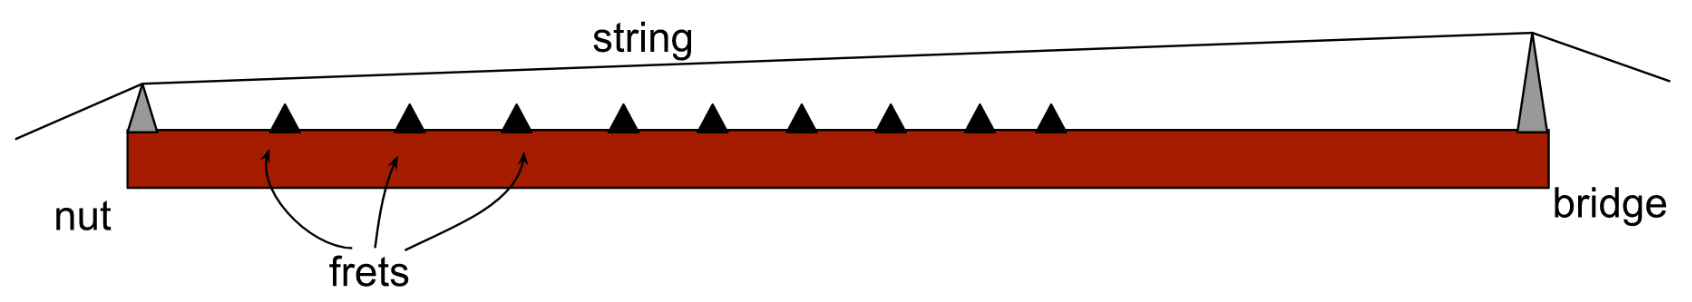
\includegraphics[width=\textwidth]{./ee/fig1.png}
    \caption{A simplified model of the electric guitar I will use. The pickup has been removed.}\label{fig1}
\end{figure} 
\FloatBarrier